\section{Interferometric products (INT / COHE / UNW \& GINT / GCOHE / GUNW)}
\label{sec:int}

The generation of the interferometric product starting from \acs{cslc} is straightforward process. It is assumed that most part of the critical processing have been solved at \acs{cslc} product generation. The only particular step to be executed during the inetrferogram generation is the split-spectrum for the estimation of the ionospheric dispersive component.

\subsection{Evaluation criteria}

\label{sec:int_criteria}

The quality of the interferometric products is evaluated by comparing the outputs generated from \acs{cslc} data with those obtained from a standard processing workflow based on original \acs{slc} data. In particular, we use the ISCE2 software package as a reference processor to generate interferograms from conventional \acs{slc} inputs. Comparison metrics include visual consistency, relative phase structure, coherence levels, and agreement in the phase. 

To assess the fidelity of the interferometric products generated directly from \acs{cslc} data, we performed a benchmark experiment using multiple SAOCOM L-band acquisitions over the Bay of Naples. One image was selected as the reference for co-registration, both in the \acs{cslc} generation pipeline and in the conventional \acs{slc}-based workflow executed with ISCE2. The remaining images were paired with this common reference, resulting in:

\begin{itemize}
  \item a set of long-temporal-baseline interferograms (master–slave separations exceeding three years), and
  \item a set of short-temporal-baseline interferograms (temporal separations shorter than 30 days).
\end{itemize}

Figures~\ref{fig:int_comparison_first} and~\ref{fig:int_comparison_pre} provide two representative examples that allow for a qualitative visual comparison between the results obtained from the \acs{cslc}-based pipeline and those generated using ISCE2. Each figure includes the following:

\begin{enumerate}
  \item \textbf{Left panel}: the wrapped interferogram generated by ISCE2 from the original \acs{slc} data.
  \item \textbf{Centre panel}: the wrapped interferogram obtained by directly applying \(\arg\!\bigl(R \cdot S^{*}\bigr)\) to the pre-generated \acs{cslc} products, where \(R\) and \(S\) refer to the reference and slave images, respectively.
  \item \textbf{Right panel}: the wrapped phase difference \(\arg\bigl(\mathrm{INT}_{\text{ISCE}} \cdot \mathrm{INT}_{\text{CSLC}}^{*}\bigr)\), used to assess potential discrepancies between the two processing chains.
\end{enumerate}

A qualitative inspection leads to the following observations:

\begin{itemize}
  \item Over land, the centre-panel phase difference is essentially flat, indicating that the interferograms produced from \acs{cslc} data are interchangeable with those generated by the well-established ISCE2 workflow.
  \item Over the sea, fringe patterns appear in the difference maps. These originate from a processing divergence rather than an error: ISCE2 embeds bathymetric information when flattening the phase before forming the interferogram, whereas the \acs{cslc}-based chain assumes a zero-elevation (sea-level) surface. Consequently, the difference field over water represents the negated bathymetric phase term included only in the ISCE2 product.
  \item No systematic residuals linked to temporal baseline length are evident, confirming that the \acs{cslc} generation has preserved the phase stability required for both short- and long-baseline interferometry.
\end{itemize}

The experiment therefore demonstrates that interferograms computed from \acs{cslc} inputs preserve the scientific quality of those generated from \acs{slc} data, while offering the processing simplifications and storage benefits inherent to the \acs{cslc} format.

\begin{figure}[ht!]
  \centering
  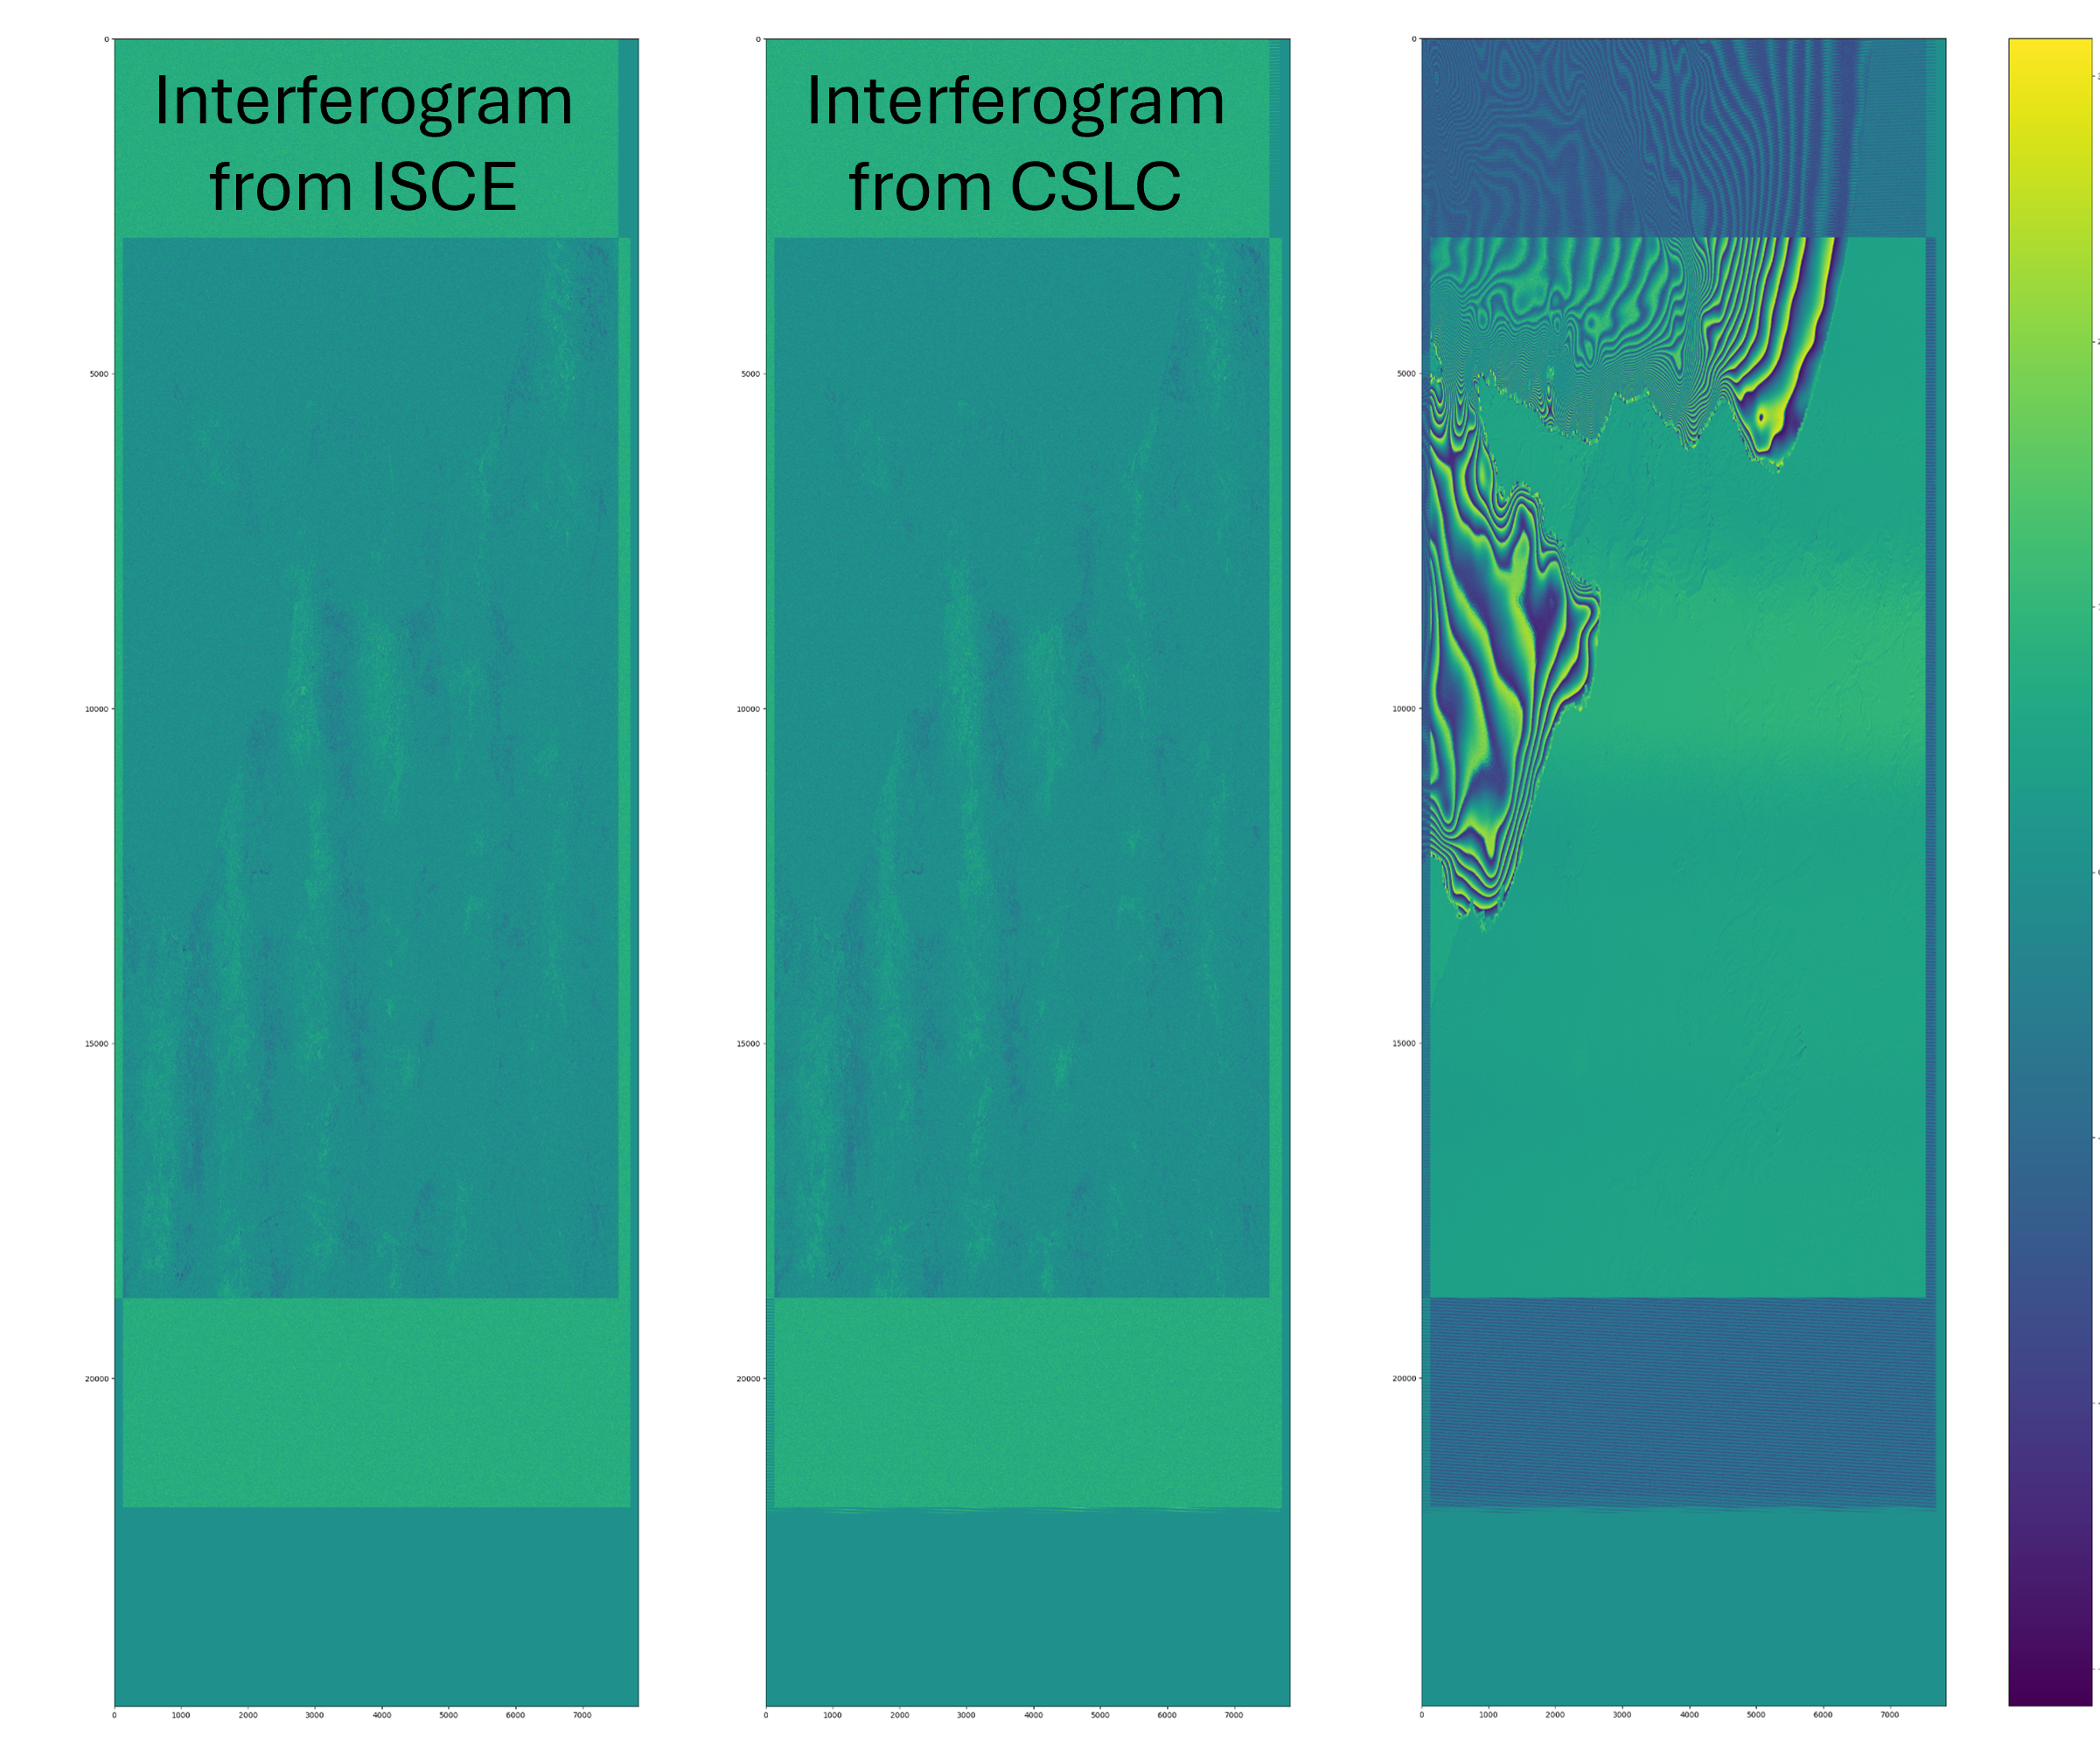
\includegraphics[width=\textwidth]{Figures/interf/comparison_first.png}
  \caption{Comparison of interferograms generated using the \acs{cslc}-based pipeline and ISCE2 for a long-temporal-baseline pair. The master image was acquired on 2023-12-12, and the slave image on 2020-04-23, resulting in a temporal separation of more than three years. Left: interferogram produced by ISCE2 from \acs{slc} data. Centre: wrapped interferogram computed directly from \acs{cslc} products. Right: wrapped phase difference between ISCE2 and \acs{cslc} results.}
  \label{fig:int_comparison_first}
\end{figure}

\begin{figure}[ht!]
  \centering
  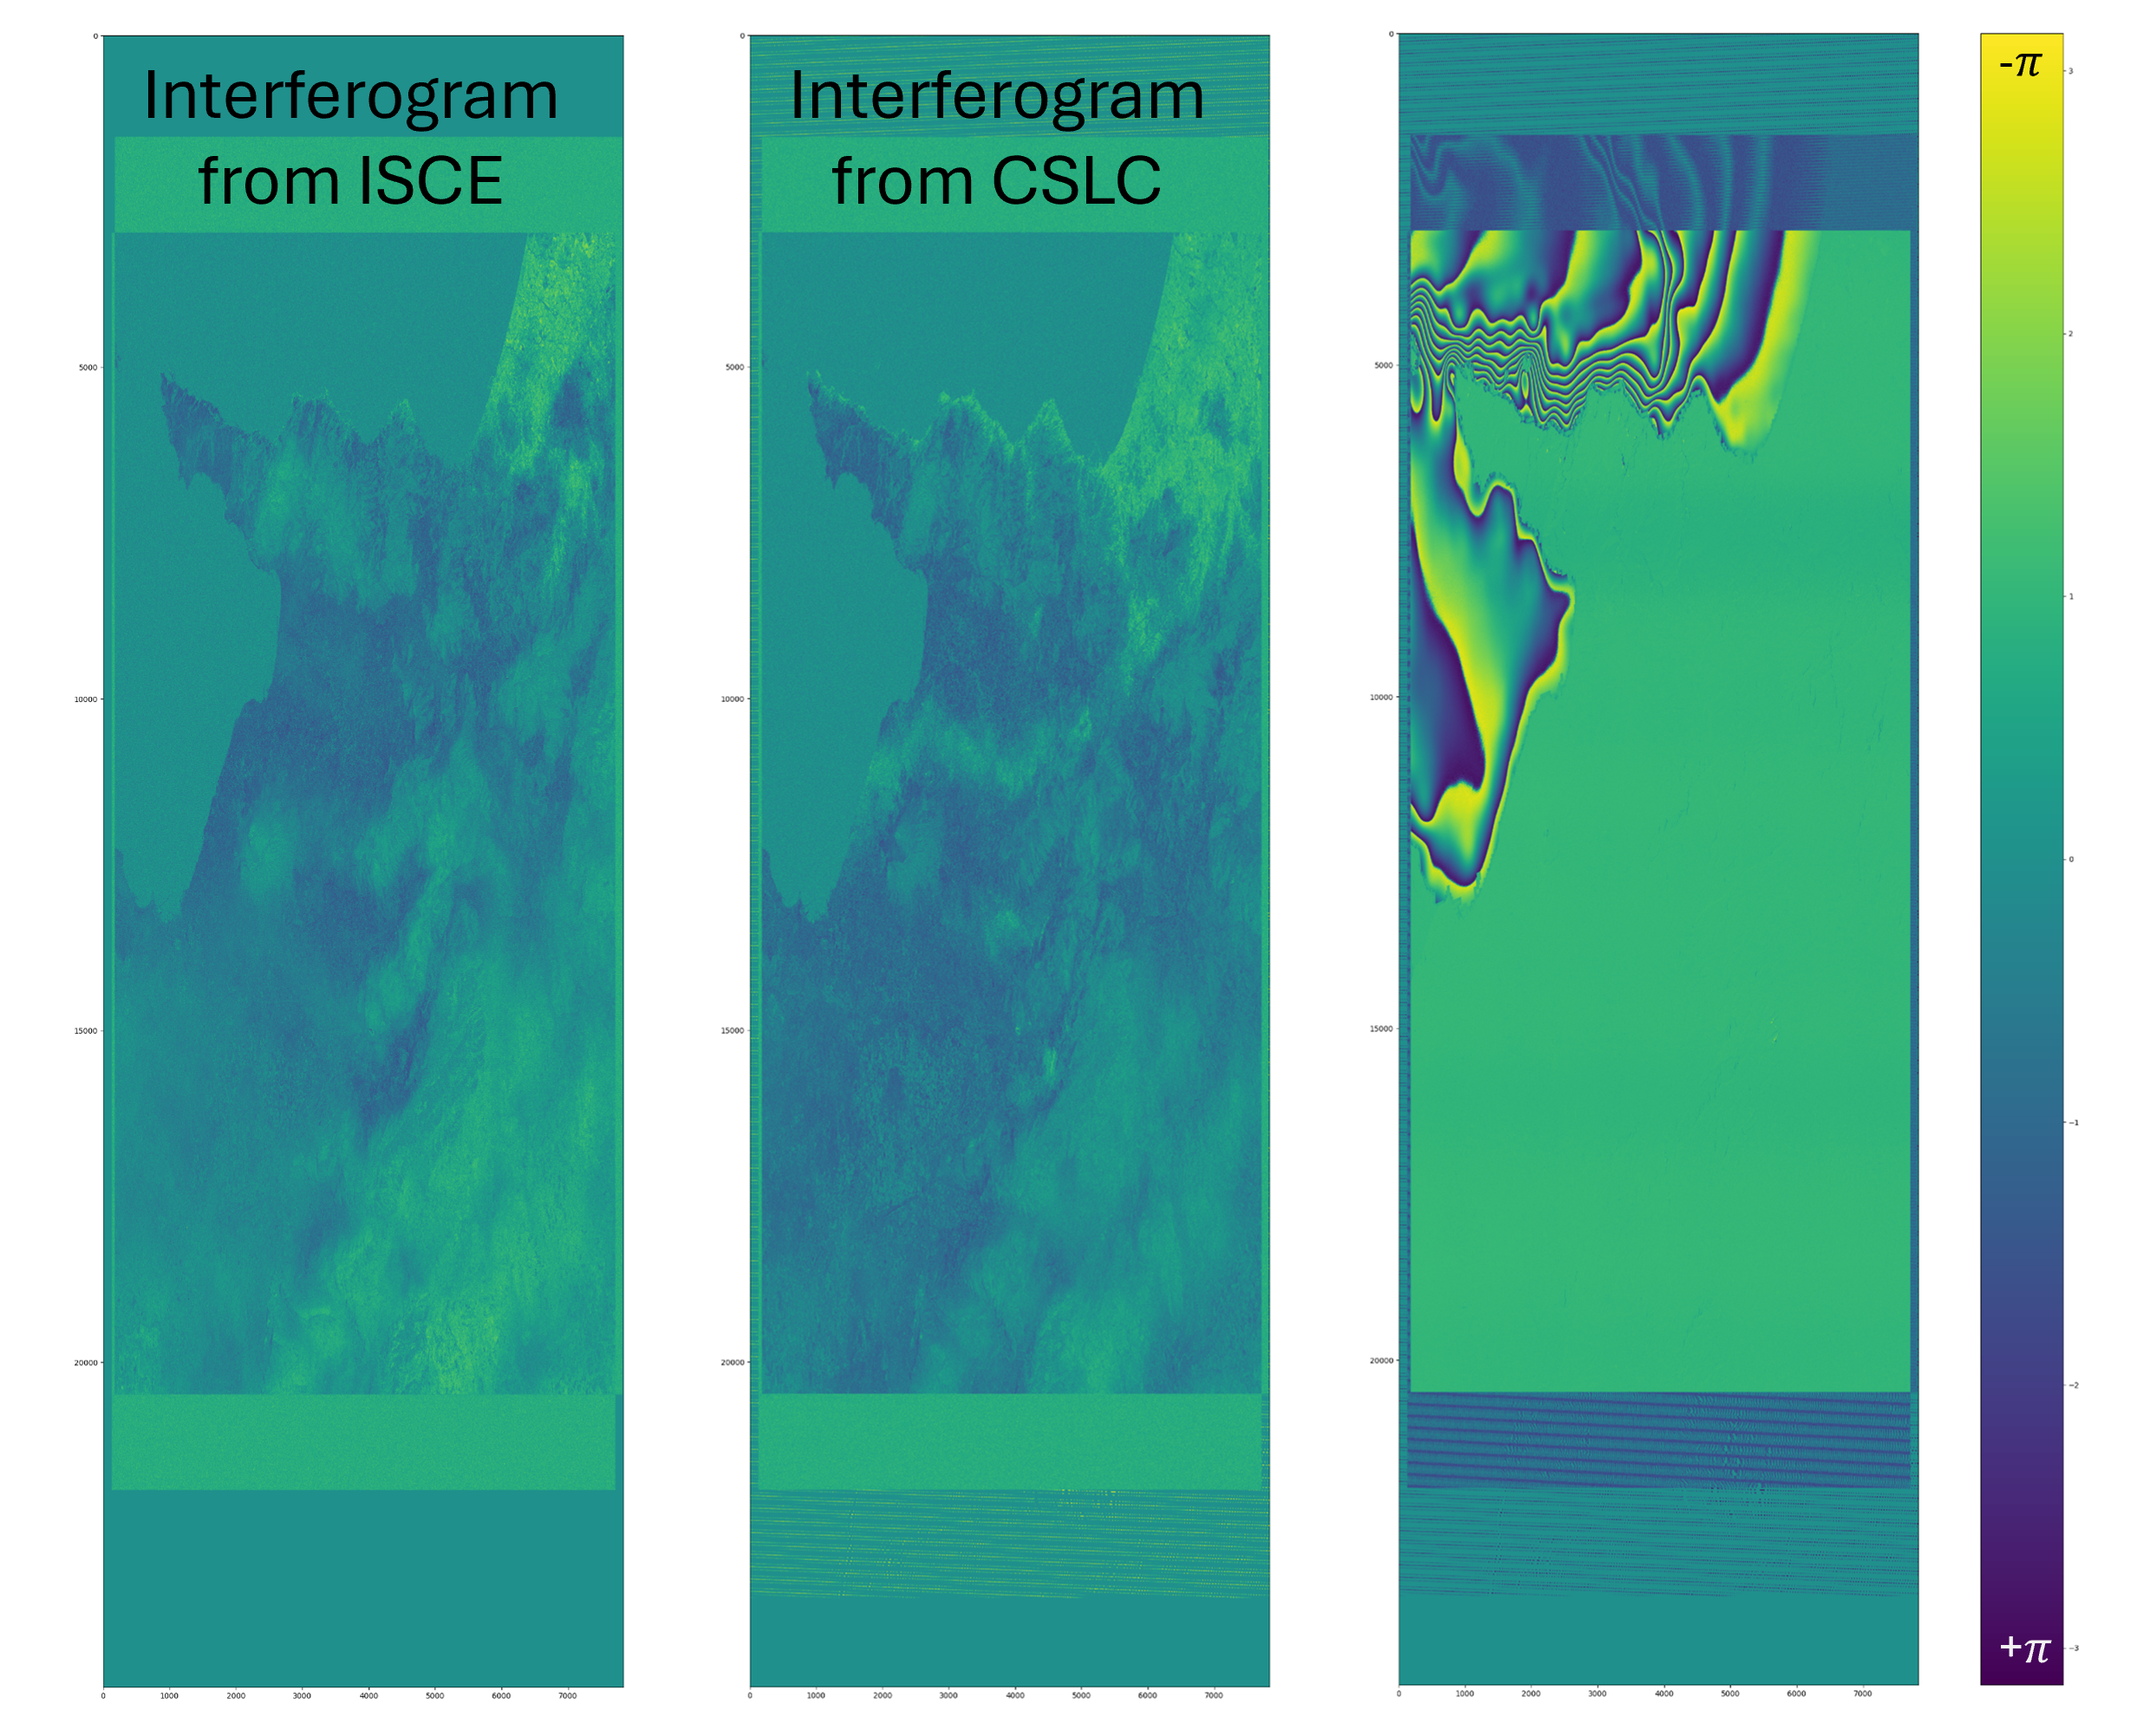
\includegraphics[width=\textwidth]{Figures/interf/comparison_pre.png}
  \caption{Comparison of interferograms generated using the \acs{cslc}-based pipeline and ISCE2 for a short-temporal-baseline pair. The master image was acquired on 2023-12-12, and the slave image on 2023-11-18, resulting in a 25-day temporal separation. Left: interferogram produced by ISCE2 from \acs{slc} data. Centre: wrapped interferogram computed directly from \acs{cslc} products. Right: wrapped phase difference between ISCE2 and \acs{cslc} results.}
  \label{fig:int_comparison_pre}
\end{figure}

In addition to the phase comparison, we also evaluated the coherence maps produced from the same image pairs. Specifically, we compared the coherence computed from the \acs{cslc}-based pipeline with that obtained using ISCE2. In both cases, coherence was estimated using square windows corresponding to approximately 100 meters in both range and azimuth directions.

Figures~\ref{fig:coh_comparison_short} and~\ref{fig:coh_comparison_long} show the results for the same two image pairs previously used for the interferometric phase analysis: one short-temporal-baseline pair (25 days) and one long-temporal-baseline pair (more than three years). Each figure consists of the following panels:

\begin{enumerate}
  \item \textbf{Left panel}: coherence map produced by ISCE2 from the original \acs{slc} data.
  \item \textbf{Centre panel}: coherence map derived from the \acs{cslc} products using the same processing parameters.
  \item \textbf{Right panel}: pixel-wise difference map, computed as (ISCE coherence) minus (CSLC-based coherence).
\end{enumerate}

The two examples clearly show that the coherence values are generally consistent between the two processing chains. Minor differences are visible, particularly in the form of horizontal striping in the difference maps, where the \acs{cslc}-based pipeline appears to yield slightly higher coherence values. This behavior suggests localized inconsistencies in the ISCE processing, which may slightly degrade coherence quality in specific areas. 

In addition, Figure~\ref{fig:coh_diff_histograms} reports the histograms of the pixel-wise coherence differences for both interferogram pairs. The histograms confirm that the differences are centered around zero and generally small in magnitude, indicating that the \acs{cslc}-based coherence maps are qualitatively equivalent to those obtained using ISCE2.

\begin{figure}[ht!]
  \centering
  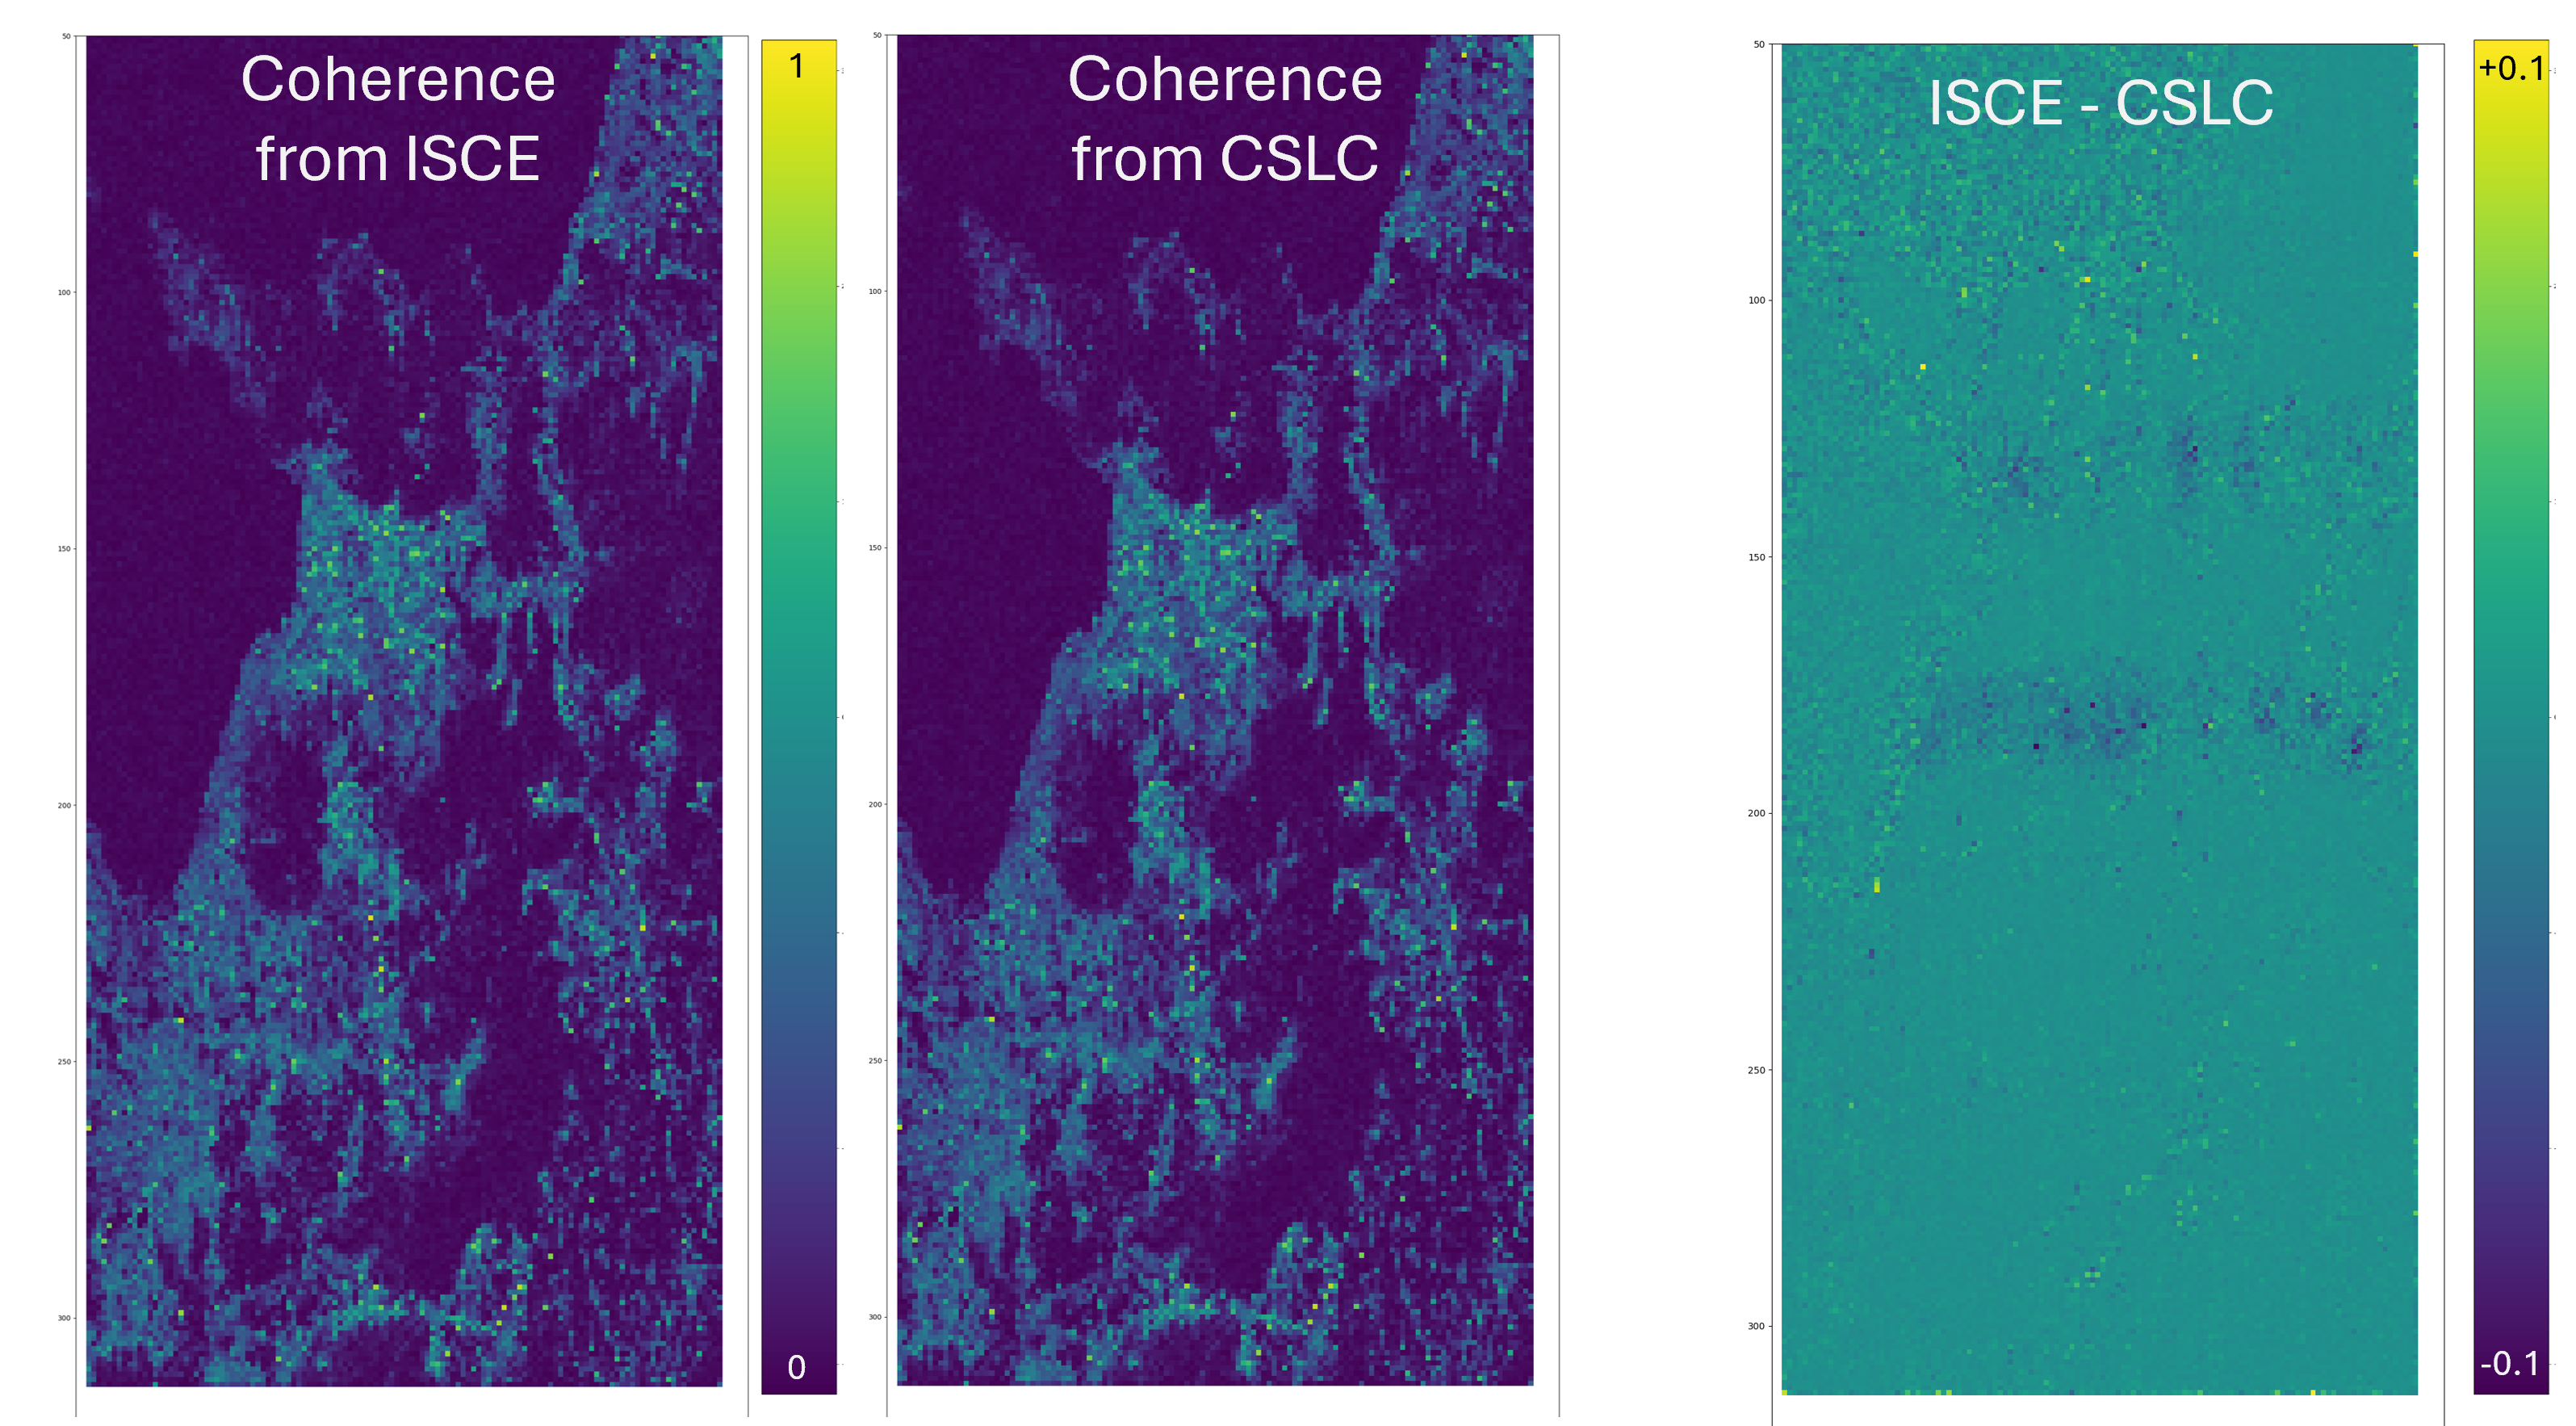
\includegraphics[width=\textwidth]{Figures/interf/coh_comparison_long.png}
  \caption{Comparison of coherence maps computed from a long-temporal-baseline image pair (more than three years). Left: ISCE2 coherence from \acs{slc} data. Centre: coherence computed from \acs{cslc} products. Right: pixel-wise difference (ISCE – CSLC).}
  \label{fig:coh_comparison_long}
\end{figure}

\begin{figure}[ht!]
  \centering
  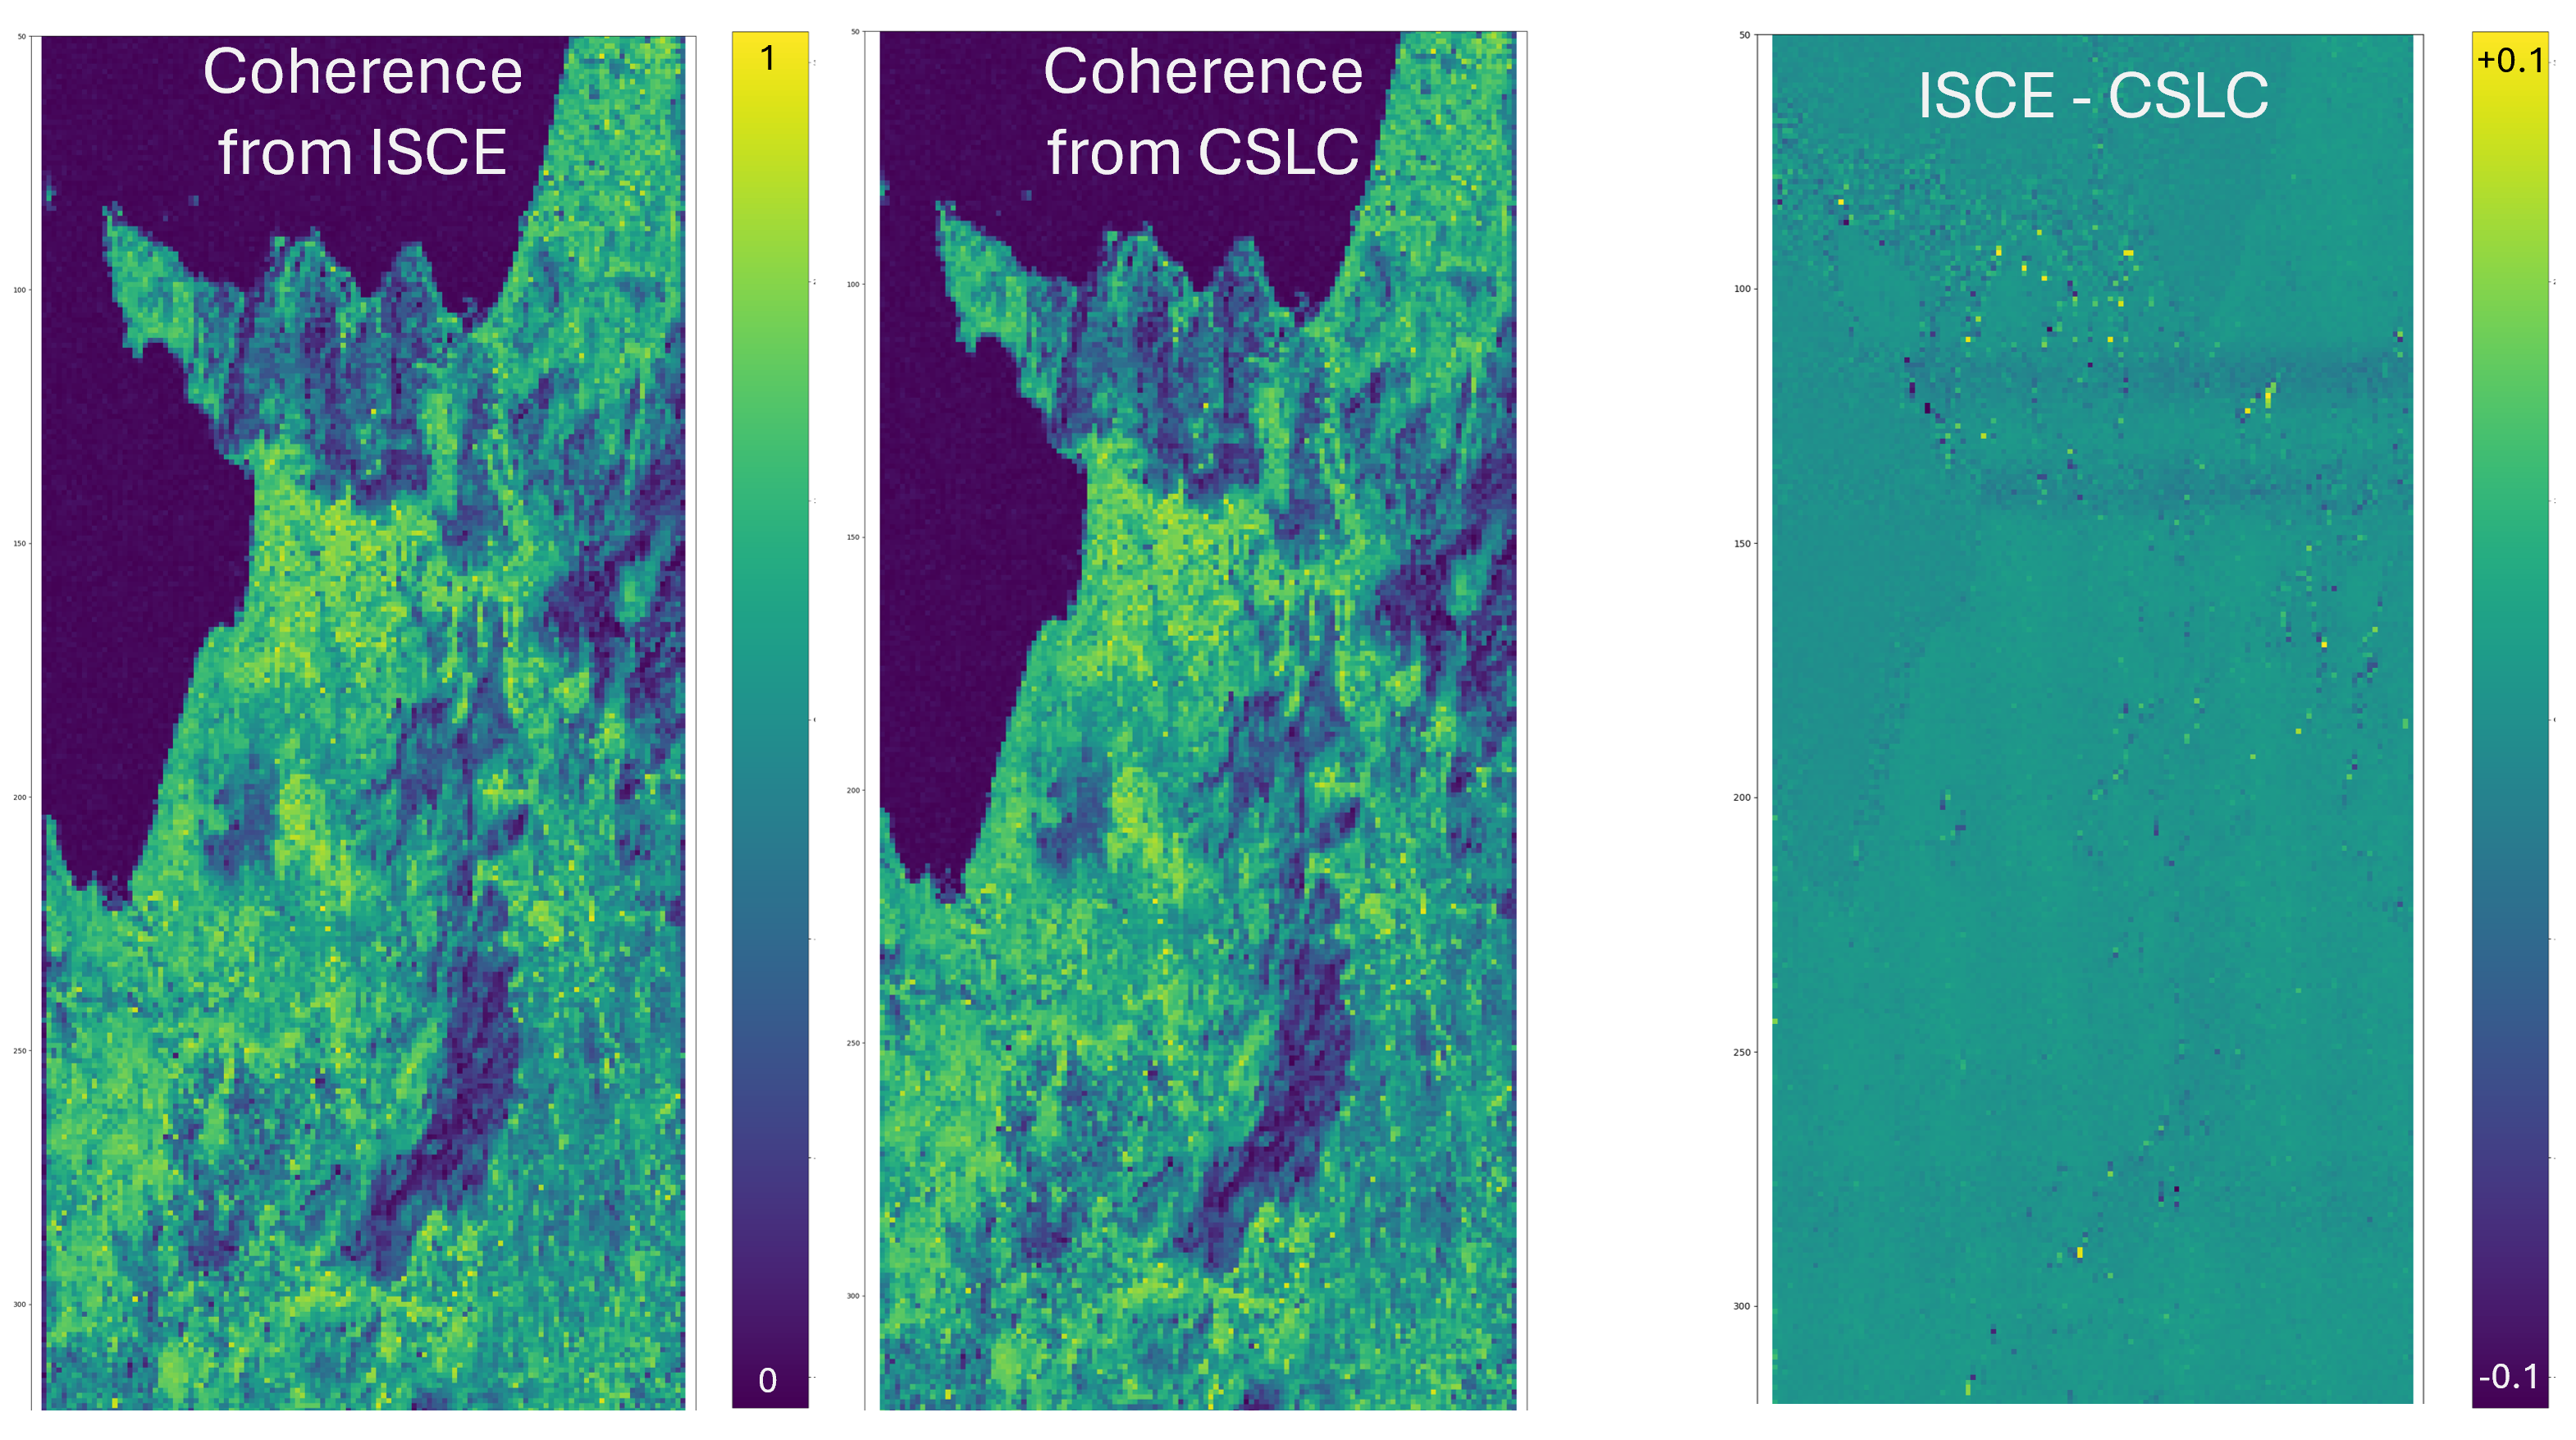
\includegraphics[width=\textwidth]{Figures/interf/coh_comparison_short.png}
  \caption{Comparison of coherence maps computed from a short-temporal-baseline image pair (25 days). Left: ISCE2 coherence from \acs{slc} data. Centre: coherence computed from \acs{cslc} products. Right: pixel-wise difference (ISCE – CSLC).}
  \label{fig:coh_comparison_short}
\end{figure}

\begin{figure}[ht!]
  \centering
  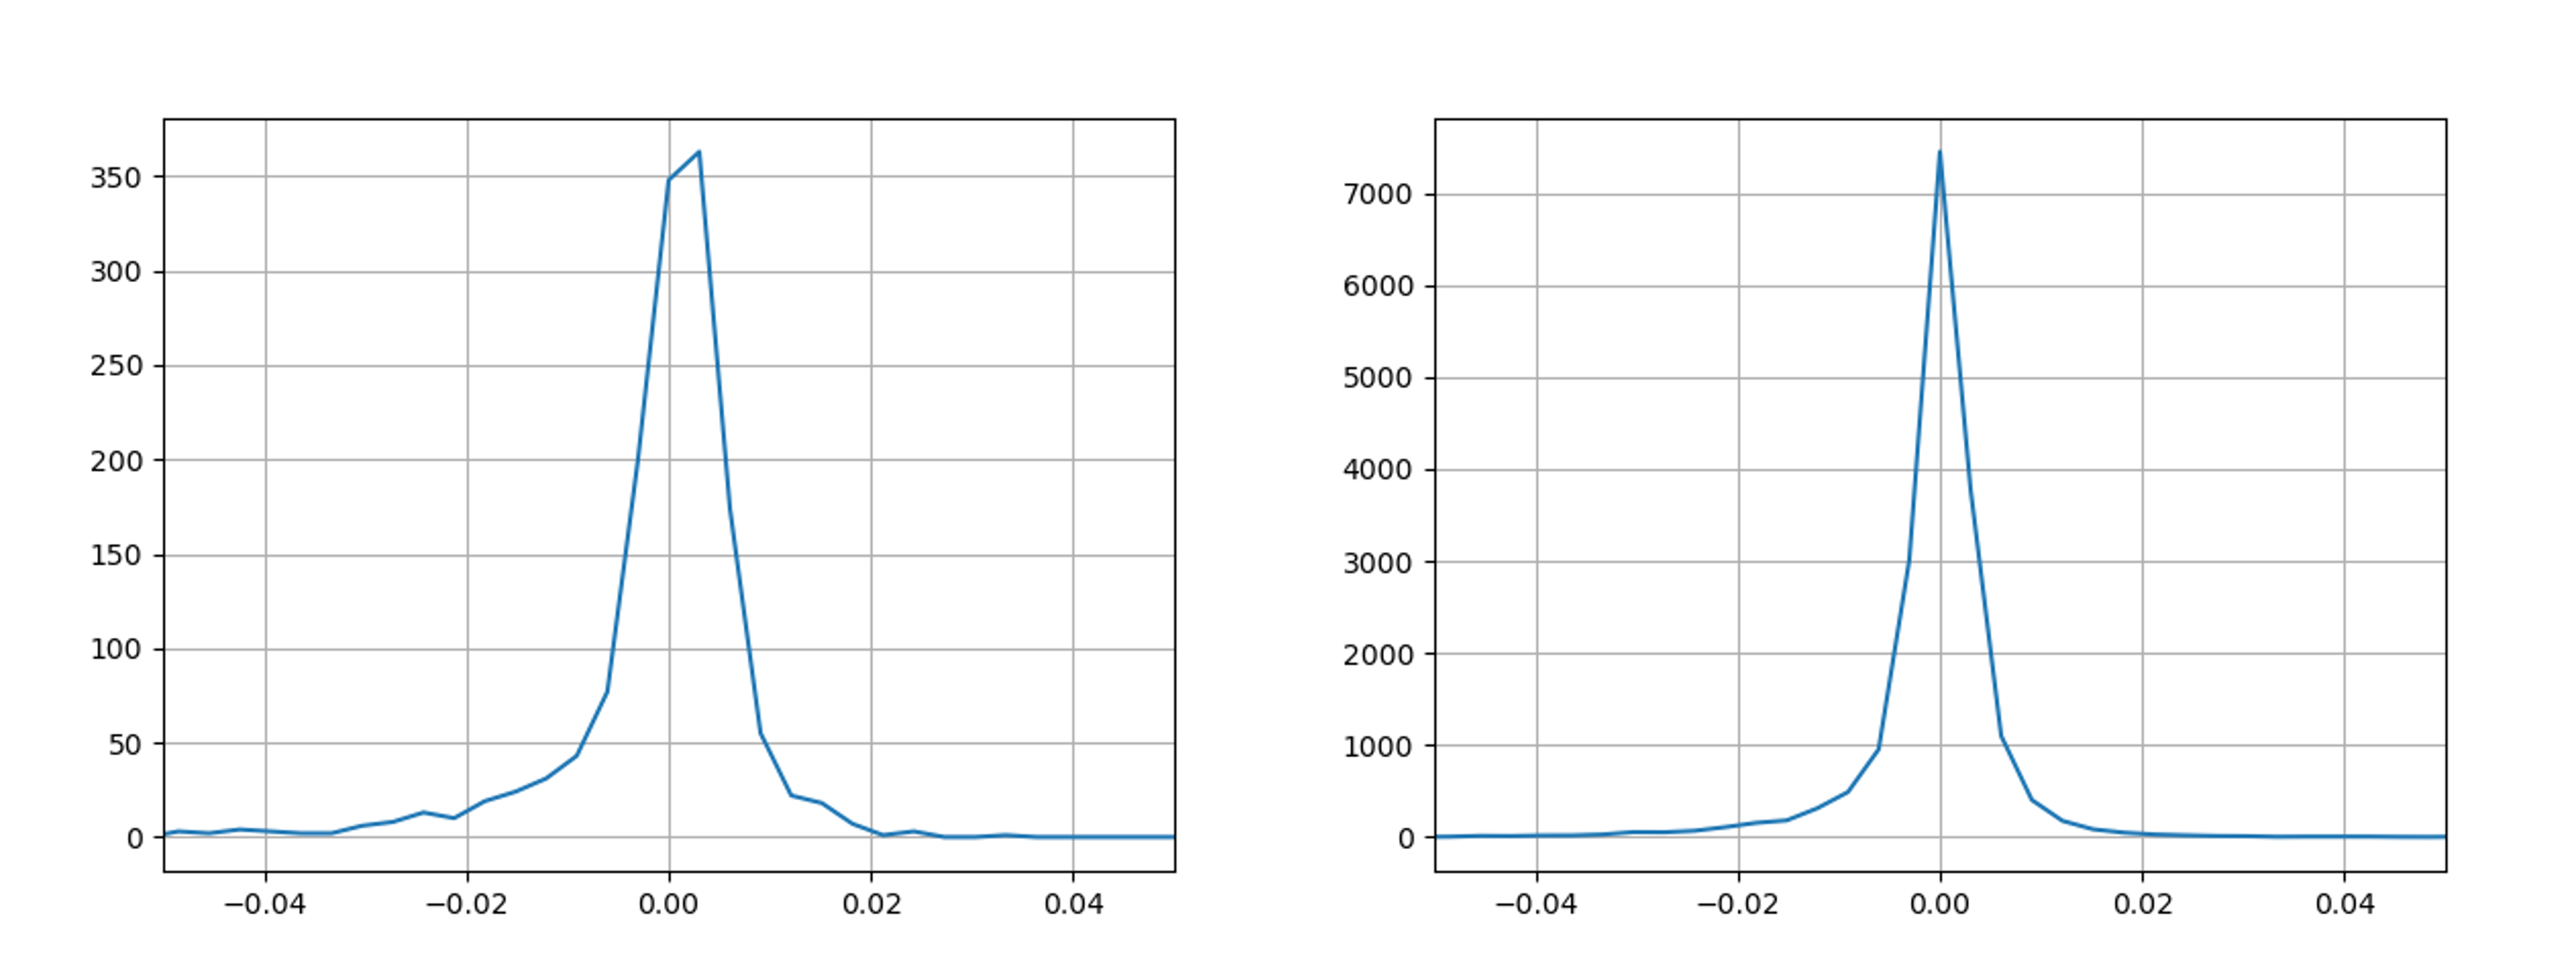
\includegraphics[width=\textwidth]{Figures/interf/istogramma_diff_first_left__pre_rigth.png}
  \caption{Histograms of the pixel-wise differences between the ISCE2 and \acs{cslc}-based coherence maps for the two image pairs (long, on the left, and short, on the right, temporal baseline). The distributions confirm that the coherence estimates from both approaches are statistically equivalent.}
  \label{fig:coh_diff_histograms}
\end{figure}

\subsection{Computational performance}
\label{sec:int_computation}
Generating the interferogram involves multiplying two complex-valued images and applying filters to reduce noise. This operation is simple, and its computational cost is proportional to the number of pixels in the input images.

The most demanding steps are split-spectrum processing and phase unwrapping. However, by using multilooked data, it is possible to significantly reduce the computational cost.

At the moment, another computationally expensive step is geocoding. This cost is the same of the \acs{nrb} product. In fact, the geocoding method is based on the same projection matrix used in the area-projection algorithm. The cost could be reduced by adopting a geocoding strategy tailored to multilooked data.

\subsection{Criticalities and weakness}
\label{sec:int_criticalities}

Interferometric products inherit the criticalities and weaknesses of the \acs{cslc} product.

\subsection{Data Generation}
\label{sec:int_data_generation}
The ISCE environment can be created using
\begin{lstlisting}[language=bash]  
conda install conda-forge::isce2
\end{lstlisting}
and the creation is performed by typing the following line:
\begin{lstlisting}[language=bash]  
yourEnv/lib/python3.11/site-packages/isce/applications/stripmapApp.py
--steps yourPath/StripmapAppSAOCOM.xml 2$>&1$ | tee SAOCOM
\end{lstlisting}
Attention must be paid in substituting \emph{yourEnv} and \emph{yourPath} with the correct paths.

Hereafter there is an example of \emph{StripmapAppSAOCOM.xml} file.

\begin{lstlisting}[language=xml]  
<?xml version="1.0" encoding="UTF-8"?>
<insarApp>
  <component name="insar">
    <property name="sensor name">SAOCOM_SLC</property>
    <component name="reference">
        <catalog>/home/debora/tests_Naples/test_pre_master/
            reference_SAOCOM.xml</catalog>
    </component>
    <component name="secondary">
        <catalog>/home/debora/tests_Naples/test_pre_master/
            secondary_SAOCOM.xml</catalog>
    </component>
    <property name="demFilename">
        <value>/home/debora/tests_Naples/demLat_40_S42_Lon_W013
            _W016.dem.wgs84</value>
    </property>
    <property name="do denseoffsets">True</property>
    <property name="do split spectrum">True</property>
    <property name="unwrapper name">snaphu</property>
    <property name="do dispersive">True</property>
    <property name="dispersive filter kernel x-size">800</property>
    <property name="dispersive filter kernel y-size">800</property>
    <property name="dispersive filter kernel sigma_x">100</property>
    <property name="dispersive filter kernel sigma_y">100</property>
    <property name="dispersive filter kernel rotation">0</property>
    <property name="dispersive filter number of iterations">5</property>
    <property name="dispersive filter mask type">connected_components</property>
    <property name="dispersive filter coherence threshold">0.6</property>

  </component>
</insarApp>
\end{lstlisting}

The \emph{dem} file can be created by typing
\begin{lstlisting}[language=bash]  
yourEnv/lib/python3.11/site-packages/isce/applications/dem.py -a 
stitch -b 39 42 13 16 -r -s 1 -c -o 
demLat_39_S42_Lon_W013_W016.dem.wgs84 --dir /yourPath
\end{lstlisting}
using the coordinates of the area of interest.




